% 以下の3行は変更しないこと.
\documentclass[T]{compsoft}
\taikai{2016}
\pagestyle {empty}

\usepackage [dvipdfmx] {graphicx}

% ユーザが定義したマクロなどはここに置く.ただし学会誌のスタイルの
% 再定義は原則として避けること.

\begin{document}

% 論文のタイトル
\title{自己調整二分木の並列操作}

% 著者
% 和文論文の場合,姓と名の間には半角スペースを入れ,
% 複数の著者の間は全角スペースで区切る
%
\author{上田 和紀
%
% ここにタイトル英訳 (英文の場合は和訳) を書く.
%
\ejtitle{Concurrent Operations on Splay Trees.}
%
% ここに著者英文表記 (英文の場合は和文表記) および
% 所属 (和文および英文) を書く.
% 複数著者の所属はまとめてよい.
%
\shozoku{Kazunori Ueda}{早稲田大学理工学部情報学科}%
{Dept.\ of Information and Computer Science, Waseda University}}

% 和文アブストラクト
\Jabstract{%
SleatorとTarjanによる自己調整二分木(splay tree)に対して並
列操作を可能にする操作アルゴリズムを提案する.提案するアル
ゴリズムは,同一の木に対する複数の更新・挿入・削除操作のパイプライン的並
列実行を許し,かつ操作系列のスループット(単位時間内に処理可能な
操作の個数)とレスポンス(個々の操作の償却計算量
(amortized complexity))を両立させることを目的としている.
スループットの最適性と挿入操作の対数的レスポンスについては
理論的結果を示す.削除操作は,木の形状に関する良い性質を保つ
にもかかわらず,Sleatorらの枠組みでは最適性が証明できない.
このことについても論じる.}

% 英文アブストラクト(本サンプルの原論文にはなし)
\Eabstract{
We propose a family of algorithms for concurrent operations on
self-adjusting binary trees (splay trees) proposed by Sleator and
Tarjan.  The goal of the algorithms is to allow pipelined execution of
multiple update/insert/delete operations while retaining good bounds
both in throughput (number of operations per unit time)
and in latency (amortized time complexity of each operation).  We show
theoretical results on the optimality of throughput of all operations
and the logarithmic latency of insert operations.  The optimality of
latency of delete operations, on the other hand, cannot be proved using
Sleator \textit{et al.}'s setting, while the operations preserve desirable
properies of the shapes of trees.}
%
\maketitle \thispagestyle {empty}

\section{はじめに}

自己調整二分木(スプレー木, splay tree) \cite{ST85}は,アクセスした節
点に対して扁平化(splaying)操作(\ref{subsection:splaying}節)
を施すことにより,木の形状を動的に最適化す
る二分探索木の総称であり,
%
% さまざまなアク
% セスパターンに対して木の形状が動的に最適化してゆく二分木であり,
%
多くの強力な性質が成り立つことがわかっている.本論文では,
同一のスプレー木に対する複数の挿入削除等の操作
のパイプライン的並列実行を可能にする方法を検討する.目標は,下記の要請を満たす
操作アルゴリズムを得ることである.
%
\begin{enumerate}
\item ({\bf レスポンス}) 通常のスプレー木の操作と同様,
対数的な償却計算量(amortized complexity)\cite{T85}をもつ.

\item ({\bf スループット}) 操作後の木の形状が,根に近い部分か
ら葉に向かって
漸増的に確定するようにすることで,個々の操作が同時に施錠しなければな
らない節点の数を高々${\rm O}(1)$個におさえる.
\end{enumerate}
%
もしスループットだけが目標ならば,二分木を用いなくても,
線形リストを用いて容
易に達成できる.したがって,レスポンスとスループット
を同時に達成することが本質的に重要である.
%
B木やその変種に対する並列操作の研究は少なくない\cite{LS86}が,スプ
レー木の並列性に関する研究は少なく,著者の知る限り,上記の二条件を満たす
並列アルゴリズムはまだ提案されていない.

本論文では,二分探索木の各節点はキーと値の対を保持するものとし,節点は
キーの対称順(symmetric order)に並んでいるとする.基本操作として,
次の二つを考える.単なる節点値の読出しは${\it update\/}$の単純な変
種と考えることができる.

\begin{description}
\item{${\it update}(i,v,v',t)$:} キー$i$をもつ節点が木$t$の中にあれば,そ
の節点の現在の値を$v$に代入したあと,節点に新たな値$v'$を格納する.
なければ,キー$i$と値$v'$をもつ節点を$t$に挿入し,$v$には節点がなかった
ことを示す特別の値を代入する.

\item{${\it delete}(i,v,t)$:} キー$i$をもつ節点が木$t$の中にあれば,その節
点の現在の値を$v$に代入したあと,節点を消去する.なければ$v$に特別の
値を代入する.
\end{description}


\section{関連研究}

\subsection{扁平化とトップダウン扁平化}\label{subsection:splaying}

スプレー木における扁平化とは,節点の探索操作において
アクセスしたパスの長さをおよそ半分にしつつ,目標
節点(${\it delete\/}$においては,目標節点の直前または直後のキーをもつ節点)
を木の根まで浮上させる操作である.扁平化は枝の回転(rotation)を基本操
作としており,図\ref{figure:splaying}に示す
zig, zig-zig, zig-zagのうちの適切な操作をボ
トムアップに繰り返す.以下本論文では,左右対称な操作群はその片方のみを示
す.また図中の小文字は節点,大文字は部分木を示す.
%
${\it update}$, ${\it delete\/}$等の個別の
操作アルゴリズムについては多くの変種がある.扁平化の大きな特徴は,アクセ
スしたパス上の各節点の深さを約半分にする一方で,アク
セスしたパスの上にない節点を,高々${\rm O}(1)$段しか深くしないこと
である.

\begin{figure}[tb]
  \centerline {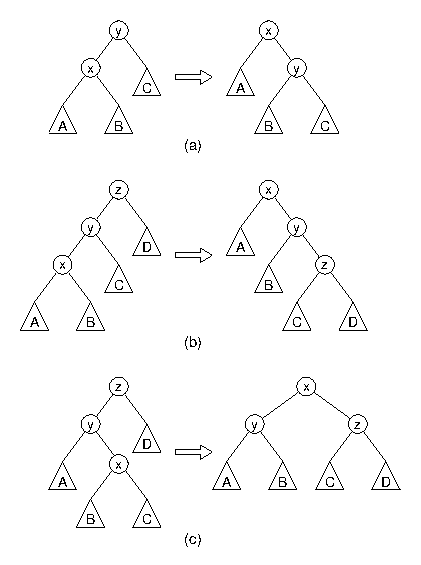
\includegraphics{images/fig1.eps}}
\caption{
ボトムアップ扁平化操作の1ステップ. % \cite{ST85}
$x$ がアクセスした節点.(a) zig: 1回の右回転($y$が根の場合
のみ),
(b) zig-zig: 枝$yz$と枝$xy$をこの順に右回転,(c) zig-zag: 枝$xy$
を左回転し,できた枝$xz$を右回転.}
\label{figure:splaying}
\end{figure}

扁平化はボトムアップな変形操作であるため,並列操作には適さない.
文献\Cite{ST85}はトップダウン扁平化も提案しているが,これは実装の
容易化が主な目的であり,木の根は操作終了の直前まで確定しない.


\subsection{並列操作に関する過去の研究}\label{subsection:related-parallel}

和田\cite{W90}は,並行論理型言語\cite{S89}の論理変数を用いた扁
平化アルゴリズムを提案している.これは,論理変数を利用して,
トップダウン扁平化をin-placeで行なうようにしたものと見なすこともできる
が,${\it update\/}$のように,対象となる節点が操作終了後の木に存在するこ
とがわかっている場合は,木の根のキーを操作の最初に確定させる点が大きな特徴で
ある.
% 
% 数百節点の連続挿入操作の並列度は4〜8であるという実験結果が
% 報告されている\cite{W90}.
%
しかしこの技法は,
${\it delete\/}$のように,操作結果の木の根が事前にわから
ない場合には適用できない.


\subsection{トップダウン扁平化の問題点}

トップダウン扁平化による${\it update\/}$は,
\ref{subsection:related-parallel}節のように
根のキーを最初に確定させるよ
うにしても,並列処理の観点からは問題が残る.たとえば,節点
$x(<b)$ ($<$はキーによる順序関係)の${\it update\/}$によって起きる
図\ref{figure:topdown}の
zig-zig操作\cite{W90} を考える($L$と$R$は,木$C$をトップダウン扁平
化した結果の左(右)部分木で,${\it update\/}$完了時までに確定).

% \begin{adjustvboxheight}
\begin{figure}[tb]
  \centerline {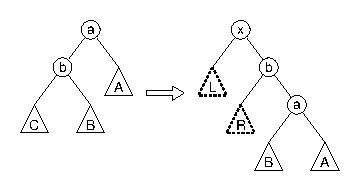
\includegraphics {images/fig2.eps}}
\caption{トップダウン扁平化による${\it update\/}$}
\label{figure:topdown}
\end{figure}
% \end{adjustvboxheight}

この${\it update\/}$の後,$y(<x)$, $z(>b)$へのアクセスがこの順に続くと
する.最初の$x$へのアクセス時に$x$が部分木$C$の左の方にあったためにzig-zig操作
が続く場合,$L$の
根が確
定するのは遅くなる.しかし$L$の根が確定するまでは,次の$y$へのアクセ
スがzig, zig-zig, zig-zagのどれをまず適用するか決められない.
% 
% 長く待っても,目標の節点の上昇段数が多ければ問題はないのであるが,
% それが
%
そこで3番目の
$z$へのアクセスが,2番目の操作によって影響を受けることのない$b$の右部分
木に向かうにもかかわらず,長時間ブロックしてしまう.

削除操作はさらに問題である.一般に,二分木から節点$x$を削除するには,
$x$の左部
分木の最大の節点$y$を探してそれを$x$の場所に移すことが基本とな
る.しかし,扁平化の有無にかかわらず,$y$が見つかるまでは$x$の場所
にくる新たなキーは確定せず,後続の操作をブロックしてしまう.以下のよう
な解決法も考えられるが,いずれもうまく動作しない.

\begin{enumerate}
\item % {\bf 一時的なキー}
$y$が見つかるまで,$x$を一時的なキーとして利用すると,
$y\le z\le x$であるような節点$z$への操作を誤った方向へ導く.

\item % {\bf 双方向リスト}
各節点が直前と直後のキーをもつ節点へのポインタを保持することによって,
$x$の直前の要素$y$に${\rm O}(1)$時間でアクセスできるようにする
ことが考えられる.これらのポインタは木
の扁平化時に変更する必要がないという特徴がある.
% 
しかしこの方法は逐次操作のときしかうまく動作しない.
% 
% あるプロセスが節点
% $x$を削除しようとしたとする.そのプロセスは節点$y$に${\rm O}(1)$時間でア
% クセスできるものの,単にそれを削除して$x$のかわりに用いることはできない.
% (invisible pointer?)
%
なぜならこの削除操作の前の操作が$x$と$y$を結
ぶパスを下降中で,いずれ$y$に到達するかもしれないからである.
\end{enumerate}

したがって本論文では,高々${\rm O}(1)$個の節を施錠しつつ,厳密にトップダウ
ンに木を変形してゆくアルゴリズムを考えることとする.

\section{並列更新アルゴリズム}\label{section:update}

本節では,後続の操作をブロックしない${\it update\/}$操作を与える.基本的な
アイデアは,zig-zigとzig-zagの両方について,目標節点をその深さの
半分までしか浮上させない半扁平化(semi-splaying)を用いることである(文献
\cite{ST85}の半扁平化は,zig-zigのみが扁平化と異なっていた).$x$を更新対
象の節点とすると,アルゴリズムは以下のようになる.
%
% ここでも左右対称な操作の片方のみを述べる.

\begin{itemize}
% \medskip\noindent (a)
\item[(a)]
空の木に対する挿入は図\ref{figure:update}
(a1)の操作,(空でない)木の根に対する更新は
図\ref{figure:update}(a2)の操作を行なう.

% \begin{adjustvboxheight}
\begin{figure*}[t]
  \centerline {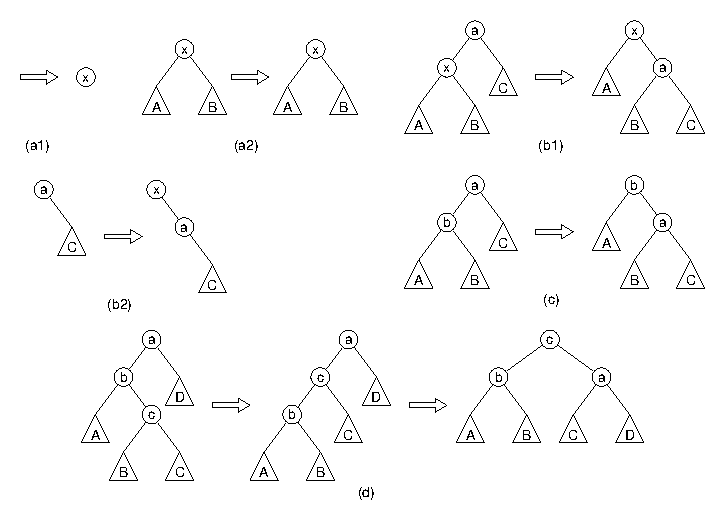
\includegraphics {images/fig3.eps}}
\caption{後続操作をブロックしない更新アルゴリズムの1ステップ}
\label{figure:update}
\end{figure*}
% \end{adjustvboxheight}

% \medskip\noindent (b)
\item[(b)]
zig: 
$x$が左部分木の根である場合は図\ref{figure:update}(b1)
の操作,$x$が存在すべき左部分木が空の
場合は図\ref{figure:update}(b2)の操作を行なう.

% \medskip\noindent (c)
\item[(c)]
zig-zig: 図\ref{figure:update}(c)左の木における$x (<b)$の探索では,
枝$ba$の右回転を行なってアクセスしたパスの長さを1短縮する.次は1レベル
(短縮前の長さでは2レベル)下降して,部分木$A$に対して再帰的に探索を行なう.

% \medskip\noindent (d)
\item[(d)]
zig-zag: 図\ref{figure:update}(d)左の木における節点$x$ ($b<x<a$) の
探索では,
枝$cb$の左回転と,できた枝$ca$の右回転を行ない,
アクセスしたパスを1短縮する.
%
% 二つの中側の部分木の適当な方に対して再帰的に探索を行なう.
%
% \noindent
$x=c$ならばこれで探索終了である.$x<c$ならば2レベル(短縮前の長さでは3レ
ベル)下降して$B$の中から$x$を再帰的に
探索する.$x>c$ならば同様に$C$の中から再帰的に探索する.$x\ge c$の場合には
枝$ca$の回転操作を省略することも考えられる.
%
$b$の右部分木が空の場合は,そこに節点$x$を挿入
したあと,上に述べた回転操作を行なう.

\end{itemize}
% \medskip
以上の操作で,アクセスしたパスの長さは最悪でも約$2/3$になる.
%
半分でなくて$2/3$なのは,上記zig-zag操作の性質によるものである.


\section{並列削除アルゴリズム}\label{section:delete}

並列削除のための基本的な着想は,扁平化操作を,削除すべき節点を下降さ
せるために利用することである.これまでは,扁平化操作はもっぱら,再度アク
セスしそう
な節点を浮上させるために用いられてきた.ここで重要なことは,削除対象の
節点以外は高々${\rm O}(1)$レベルしか下降させないようにすることである.
以下では,$z$を削除対象の節点とする.

まず,根節点が削除対象節点$z$である場合を考える.この場合,zippingと呼ぶ
操作によって
それを``容易に''削除できる場所まで下降させる.節点が``容易に''削除でき
るとは,その左部分木,右部分木,左部分木の右部分木,右部分木の左部分木の
いずれかが空であることである.根節点の下降によって,その左部分木と
右部分木の縫い合せが起きる.
% 
% これが言葉の由来である.

\begin{enumerate}
% \medskip\noindent (a)
\item[(a)]
``容易に''削除できる場合:図\ref{figure:delete}(a1)または(a2)
のように変形する.


% \begin{adjustvboxheight}
\begin{figure*}[t]
  \centerline {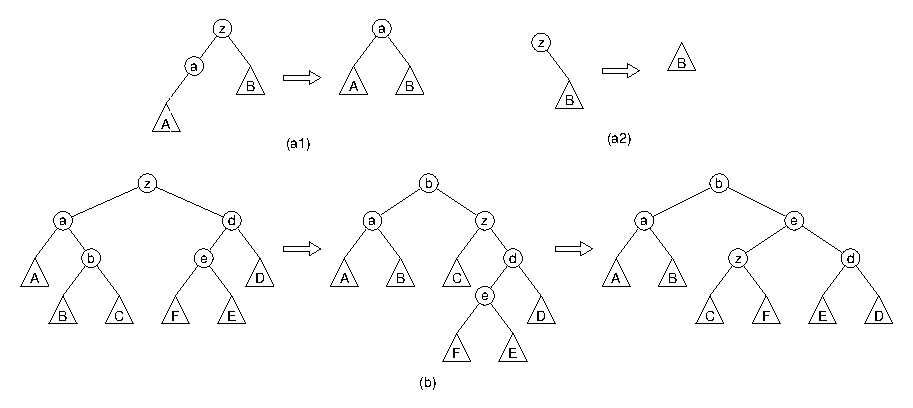
\includegraphics {images/fig4.eps}}
\caption{後続操作をブロックしない削除アルゴリズムの1ステップ}
\label{figure:delete}
\end{figure*}
% \end{adjustvboxheight}

% \medskip\noindent (b)
\item[(b)]
``容易に''削除できない場合:図\ref{figure:delete}(b)のように
zig-zagを施し,そ
の結果できる$b$の右部分木に,(一つめとは左右対称な) zig-zagを施す.

\noindent
4回の回転で$z$は2レベル下降する.$z$の新たな部分木$C$と$F$
は,同じレベルにとどまる.それ以外の節点も高々1レベルしか下降
しない.$z$を根とする新たな部分木に対して再帰的に削除操作を行なうが,$z$の子孫
でない節点がそれによってさらに下降することはない.
\end{enumerate}

% \medskip
図\ref{figure:zipping}に,根節点$z$の削除による木の形状の変化を示す.
\begin{figure*}[t]
  \centerline {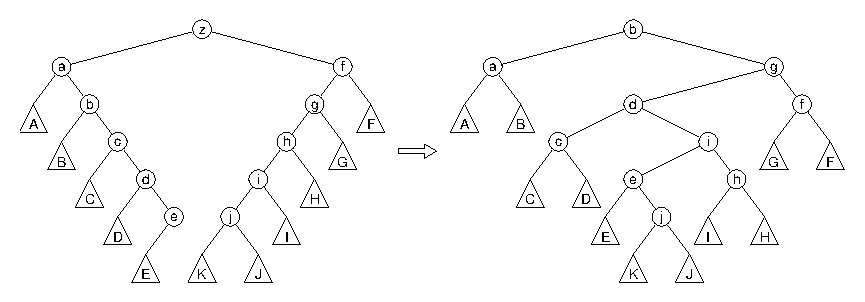
\includegraphics {images/fig5.eps}}
\caption{Zippingによる節点$z$の削除}
\label{figure:zipping}
\end{figure*}

削除対象節点$z$が根であるとは限らない場合は,まず第\ref{section:update}節の
方法で$z$を探索する.これは根から$z$に至るパスを短縮する効果をもつ.つぎ
に,$z$をzippingによって下降させて削除する.

Zipping操作はパスの短縮を行なわないが,アクセスした節点は浮上させ
るという原則にしたがうならば,zippingに先だって,左部分木の最大要素に至
るパスと右部分木の最小要素に至るパスをそれぞれトップダウンの半扁平化
(zig-zig (図\ref{figure:update}(c)) の繰返し)によっ
て短縮すればよい.この短縮化はzippingと並行して行なうことができる.

Zippingは更新操作と異なり,各節点のキー値を読むことなく木を下降する.
またzippingは,木$T_1$と木$T_2$ ($T_1$のど
のキーも,$T_2$のどのキーよりも小さいものとする)とのトップダウン併合操作
にも応用できる.すなわち,新たな節点(キーは任意)を調達し,その左部分木
を$T_1$,右部分木を$T_2$として一つの木を構成した
のち,調達した根節点を消去すればよい.

\section{計算量に関する結果と考察}

効率の二つの尺度のうち,スループットにつ
いては容易に議論ができる.すなわち,二つの操作は,レベル$l$ (根をレ
ベル$0$として)の節点を${\rm O}(l)$回 --- ${\it update\/}$は高々$(l+2)$回,
zippingは高々$(2l+2)$回 ---
の回転操作ののちに確定させる.
さらにどちらの操作も,連続する高々$3$
レベルの節点を同時に施錠するだけでよい.これらのことから,木の大きさや深
さによらないスループットで,操作系列をパイプライン的に並列処理するこ
とができる.

レスポンスは,${\it update\/}$については,通常のスプレー
木と同等の償却計算量をもつことが証明できる.具体的には,
節点$x$の{\bf 大きさ}$s(x)$を$x$を根とする部分木の節点数と定義し,
{\bf ランク}$r(x)$を$\log_2(s(x))$とする.
そして
%
木の{\bf ポテンシャル}を,すべての節点のランクの和と定義する.
すると,${\it update\/}$の償却時間,つまり回転操作の回数で測った所
要時間に操作前後のポテンシャルの変化を加えたものは,$n$を木の節点数とし
て,${\rm O}(\log n)$であることを示すことができる.
このことから,十分長い操作系列の平均レスポンスは,最悪でも対数的であるこ
とがわかる.
文献\Cite{ST85}のよう
に,節点に異なる重みをつけて$s$や$r$を定義することにより,より強い性質
を示すこともできるが,本論文では省く.

一方,${\it delete\/}$については,文献\Cite{ST85}の解析方法では,対
数的償却計
算量を導くことはできない.そのことを示すために,図\ref{figure:delete}
(b)の4回の回転によるポテンシャル変化を考える.

図\ref{figure:delete}(b)の一番右側
の木のランク関数を$r'$とする.一番左側の木からのポテンシャルの変化を,
$k$をある正定数として$k(r'(b)-r'(z))$以内に押さえることができることを示すのが,
文献\Cite{ST85}における償却計算量の証明技法の基本であった.しかし,
これらの木に
ついて$s(A)= s(B) = s(C) = h\gg t = s(D) = s(E) = s(F)$
を仮定すると,ポテンシャル変化が$h/t$に関して${\rm O}(\log
(h/t))$となる.一方$r'(b)-r'(z)$は$h/t$に関して${\rm O}(1)$であるので,
上記の要請を満たす
$k$は存在しないことがわかる.Zippingに先立ってパス短縮化を行なっ
た場合についても,同様のことが示せる.

しかし,第\ref{section:delete}節の削除操作は,
%
アクセスしたパス上の節点の深さが約半分になり(事前にパス
短縮化を施した場合),それ以外の節点も高々定数レベルしか沈まない
%
という,節点の浮き沈みについてのスプレー木一般の性質は満たしている.
%
では一般に,この二つの性質を満たす自己調整的な木アルゴリズムで,平均レス
ポンスが対数時間で押さえられないような,十分長い操作系列は存在す
るのだろうか? これは未解決であるが,本論文で提案した二操作に
ついては,平均レスポンスは少なくとも${\rm O}(\sqrt n)$ (更新のみならば
${\rm O}(\log n)$)と予想される.

その根拠
として,各節点の削除しやすさの変化を考える.
節点$x$の{\bf 削除困難度}$d(x)$を,$x$からその直前のキー$x_-$をもつ節
点へ至るパス長($x_-$が存在しない場合や,$x_-$が$x$の子孫で
ない場合は$0$と定める)と直後のキー$x_+$をもつ節に至るパス長の最小値
と定めると,第\ref{section:delete}節の
${\it delete\/}$は,$d$の大きな節点の消去には時間がかかるも
のの,残った各節点の$d$を高々${\rm O}(1)$
しか大きくしない.また第\ref{section:update}節の
${\it update\/}$で新たに挿入した節点の$d$
は$0$であり,${\it update\/}$はすでに存在していた各節点の$d$も高々${\rm
O}(1)$しか大きくしない.(ボトムアップ扁平化における節点の$d$の増加は,定数で
押えることができない.)これらのことから
%
\begin{enumerate}
\item[1.]
新たな節点の$d$の値が$k$まで成長するには,他の節点の$\Omega(k)$
回の挿入削除が必要
\end{enumerate}
%
であることがわかる.さらに
%
\begin{enumerate}
\item[2.]
二分木における各節点の$d$の総和は,
木をトラバースしたときに通る枝の延べ本数を上回ることはないから
${\rm O}(n)$
\end{enumerate}
%
である.1.と2.から,
新たな節点の挿入と,$d$の大きな節点の消去が繰り返されるという最悪の操作
系列を考えても,操作の平均の手間は${\rm O}(\sqrt n)$であり,実用上の効率
は更新操作のみの場合とほとんど変わらないと予想される.

\section{まとめと今後の課題}

節点の浮き沈みに関する望ましい性質を保ち,かつ計算量の意味で最適なスルー
プットをもつ自
己調整二分木の並列操作(更新,挿入,削除,併合)アルゴリズムを提案した.節点の
更新や挿入に関して
は対数的償却計算量を持つことが証明できており,さらにアクセスパターンの偏
りや変化に対する追従性など,スプレー木の持つ強力かつ頑健な性質
の多くを引き継いでいる.削除の償却計算量のより良い理論的限界を導く(また
はその不存在を示す)ことは今
後の課題である.また,アルゴリズムの実際的効率,並列分散環境での実装,応
用の検討も今後の課題である.


{\bf 謝辞}\
本論文の初期の版について議論していただいたRobert Tarjan氏(Princeton大),
毛受哲氏(NEC),中谷祐介氏(早稲田大)に感謝する.

\bibliographystyle {jssst}
\bibliography {sample}

\appendix
\section{付録: \LaTeX による論文作成のガイド} 

ここに,以前の \verb|sample.tex| では,論文作成のガイドがあったが,
その内容は \verb|guide.tex| に移動した.
\verb|guide.tex| は,スタイルファイル配布物一式の中に含まれている.

\end{document}
